\documentclass{article}
\usepackage[english]{babel}
\usepackage[final,nonatbib]{nips_2017}
\usepackage[utf8]{inputenc} % allow utf-8 input
\usepackage[T1]{fontenc}    % use 8-bit T1 fonts
\usepackage{hyperref}       % hyperlinks
\usepackage{url}            % simple URL typesetting
\usepackage{booktabs}       % professional-quality tables
\usepackage{amsfonts}       % blackboard math symbols
\usepackage{nicefrac}       % compact symbols for 1/2, etc.
\usepackage{microtype}      % microtypography
\usepackage{graphicx}
\usepackage{appendix}
\usepackage[backend=biber, style=numeric, citestyle=numeric]{biblatex}
\usepackage{longtable}
\addbibresource{references.bib} %Imports bibliography file

\title{Long Short-Term Vehicle Dynamics}
\author{
  David Casterton\\
  Stanford University, CS230 Spring 2019\\
  \texttt{david.casterton @stanford.edu / @gmail.com} \\
}

\begin{document}

\begin{center}

\includegraphics[width=3cm, height=0.7cm]{CS230}
\end{center}

\maketitle

\begin{abstract}
Vehicle dynamics simulation can achieve excellent results from manually crafted physical models, however manually crafting models can be time consuming, financially and computationally expensive, difficult to tune details, and difficult to generalize. This project focused on potential roles of Deep Neural Network's (DNNs) to improve vehicle dynamics simulation by utilizing data to learn the model.
\end{abstract}

\section{Introduction}	
A key challenge to bringing autonomous vehicles to market is proving they can safely operate within a very large state space of potential scenarios and associated sensor inputs. Simulation is one of the leading techniques being pursued to make this proof, due to the promise of scalable parallelization for rapid feedback and eventual deep exploration of the operational state space. However, before a simulator can meaningfully inform how a specific real-world vehicle will perform, the accuracy of the simulation must be well understood and refined to be within acceptable bounds.

This project evaluated if simulated vehicle movement can be improved by learning unmodeled attributes from vehicle specific data. Results show that training Long Short Term Memory (LSTM) Recurrent Neural Networks (RNN) for end-to-end learning of vehicle movement can output next movements with plausible results for some movement features, but that end-to-end learning results alone do not appear to outperform physics modeling. LSTM experiments were performed with the input of variable lengths of recent history from vehicle movement and control, and output as the next update for vehicle movement. Related work indicates that joint usage of physics modeling and novel LSTM architectures can achieve better results than physics modeling alone.

\section{Related work}

\cite{guiggiani2014science, jazar2017vehicle, popp2010ground, schramm2014vehicle} are examples from the mature field of vehicle dynamics modeling, which yields excellent results however is limited by the manual effort put in to the physical modeling. \cite{bojarski2016end} explores end-to-end Deep Learning (DL) all the way from camera pixels to vehicle actuation output, this does not focus specifically on vehicle dynamics but presents a surprisingly successful extreme for the limit of end-to-end DL in vehicles. \cite{shi2018neural, zeng2019tossingbot} present techniques to unify physics models with DNN's, with results outperforming physics models alone. \cite{shi2018neural} specifically presents a nominal dynamics model combined with a DNN to learn how to control multi-rotor drone movement and landing, which utilizes modeling for the well known aspects of the problem then extends modeling with a DNN resulted in better performance than a baseline control system.

\section{Dataset and Features}

Data for this project was acquired from \cite{revs_vehicle_dynamics_database}, which contains 22 files of vehicle dynamics recorded from an expert driving a 1965 Ferrari in 2013 and 2014 at \textit{Monterey Motorsports Reunion} and \textit{Targa Sixty-Six} events. This data set includes the notable features of: physical inputs to the vehicle (steering, brake, throttle, clutch), GPS position (latitude, longitude, altitude), velocity and acceleration of the center of gravity (x, y, z), orientation angle and rate (roll, pitch, yaw), accuracy of position and orientation, vertical chassis accelerations, suspension deflections, and wheel accelerations.

\begin{figure}[h!]
  \centering
  \begin{minipage}[b]{0.49\textwidth}
    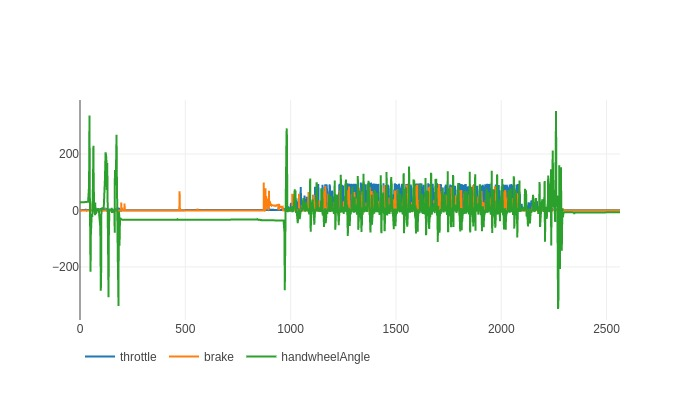
\includegraphics[width=\textwidth]{20130810_01_01_01_grandsport-0-None-100-313a19e.jpeg}
    \caption{Steering, brake, throttle from 2013.}
    \label{fig:trace1}
  \end{minipage}
  \hfill
  \begin{minipage}[b]{0.49\textwidth}
    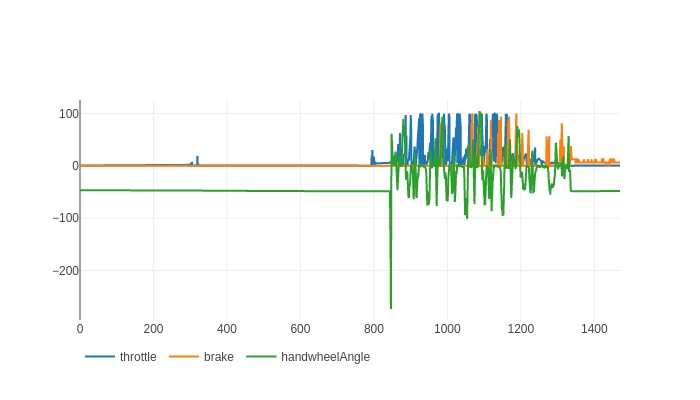
\includegraphics[width=\textwidth]{20140221_03_02_03_250lm-0-None-100-313a19e.jpeg}
    \caption{Steering, brake, throttle from 2014.}
    \label{fig:trace2}
  \end{minipage}
\end{figure}

Figures \ref{fig:trace1} and \ref{fig:trace2} show zoomed-out examples of full files, which indicate idle time at the start and end of files, with repeated maneuvers in the middle from race laps.

\begin{figure}[h!]
  \centering
  \begin{minipage}[b]{0.49\textwidth}
    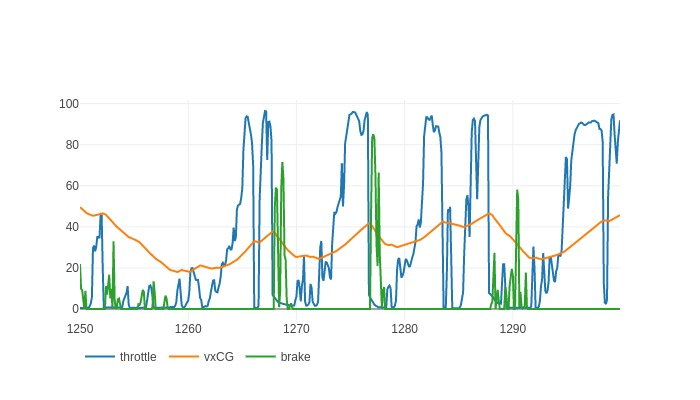
\includegraphics[width=\textwidth]{20130810_01_01_01_grandsport-12500-13000-1-cd12f64.jpeg}
    \caption{Zoomed-in longitudinal signals.}
    \label{fig:longitudinal}
  \end{minipage}
  \hfill
  \begin{minipage}[b]{0.49\textwidth}
    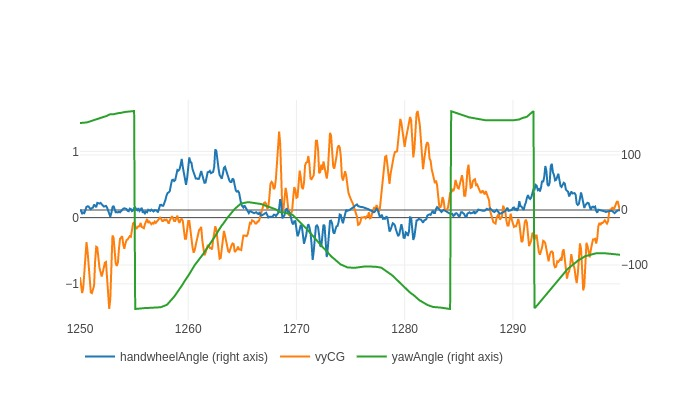
\includegraphics[width=\textwidth]{20130810_01_01_01_grandsport-12500-13000-1-9103b57}
    \caption{Zoomed-in lateral signals.}
    \label{fig:lateral}
  \end{minipage}
\end{figure}

Figures \ref{fig:longitudinal} and \ref{fig:lateral} show zoomed-in example data from the data set with strong correlations. Figure \ref{fig:longitudinal} shows that throttle and brake have a strong correlation with longitudinal velocity (vxCG). Figure \ref{fig:lateral} shows that hand wheel angle has a strong correlation with lateral velocity (vyCG) and yaw angle, however these correlations have some unintuitive attributes: hand wheel angle has an inverted sign from lateral velocity (vyCG), and yaw angle has a discontinuity at +/-180 where it inverts its sign.

This data set was recorded at 1000 Hz, however since some signals only update at 100Hz I chose to sample the data for training with a stride of 10. Some signals I considered critical (velocity, acceleration, orientation) appear to have originated from a GPS sensor that occasionally stopped updating, which resulted in those signals being temporarily incorrect then jumping with a discontinuity. To sanitize GPS discontinuities from this data set all rows were removed that contained \textit{null} for GPS altitude.


\section{ Methods }

\subsection{Hand engineering features into data}

The initial method pursued was to hand engineer features into the input data set that were considered to optimize for learning. The hypothesis was to train a neural network using all input columns available to output the change in position and orientation for the next time step. To accomplish this additional columns were appended to input data with the discrete derivatives of position and orientation between the current time \textit{t} and \textit{t+1}. Then to avoid the idle times shown in Figures \ref{fig:trace1} and \ref{fig:trace2} disproportionately impacting the training, dev, or test set, all rows were shuffled to create an equal distribution across a file. Once a file had an equal distribution the rows were split 90\% training, 5\% dev, 5\% test, then the columns were separated so original columns became input features and the new discrete derivatives became output labels.

Sequential TensorFlow models composed of a variable number of dense layers were trained against the data strategy described above, with limited success. After spending more time with the data it became apparent that this strategy was not adequately accounting for the delay between human inputs (steering, brake, throttle) being given to the vehicle and the resulting actuation (motor, brake, steering response) - training against labels for the discrete derivative of the next time step only did not give adequate time for the input to result in a learnable actuation response. A brief attempt was made to hand engineer features with longer input/output relationships, however this was quickly abandoned in favor of pursuing a network architecture that could learn temporal sequences.

\subsection{Long Short-Term Memory Recurrent Neural Networks}

To handle the problem of unknown temporal delays between vehicle input and output actuations, a RNN was chosen due to its ability to make decisions from a temporal sequence \cite{karpathy2015}, with the hope that would enable relationships to be learned with unknown temporal delays.

\begin{figure}[h!]
  \centering
  \begin{minipage}[b]{0.49\textwidth}
    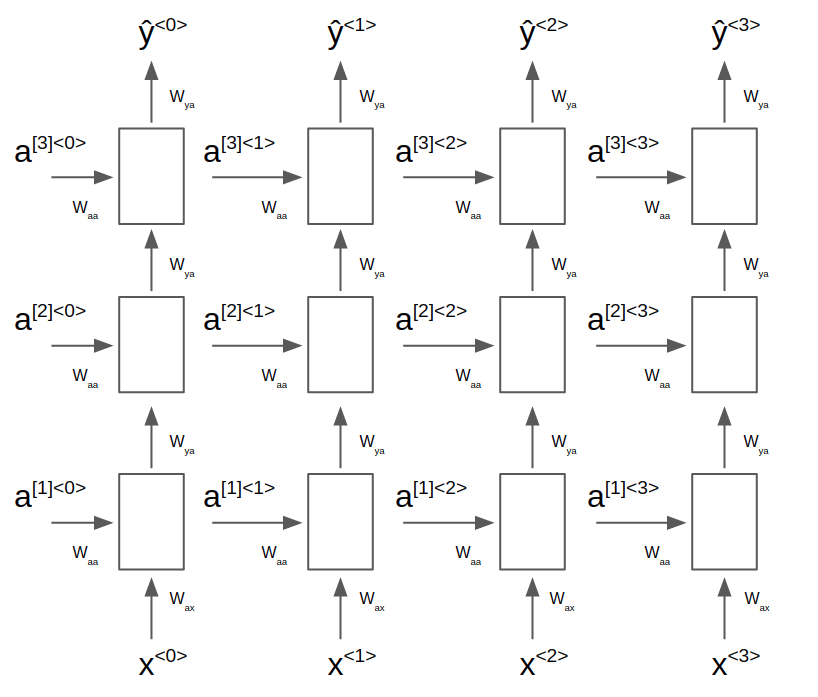
\includegraphics[width=\textwidth, height=4.75cm]{LSTM_arch}
    \caption{LSTM network architecture.}
    \label{fig:LSTM_arch}
  \end{minipage}
  \hfill
  \begin{minipage}[b]{0.49\textwidth}
    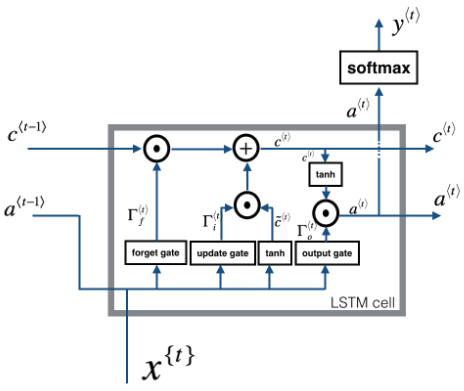
\includegraphics[width=\textwidth, height=4.75cm]{LSTM_cell}
    \caption{LSTM cell from \cite{ng_katanforoosh_bensouda_mourri}}
    \label{fig:LSTM_cell}
  \end{minipage}
\end{figure}

Figures \ref{fig:LSTM_arch} and \ref{fig:LSTM_cell} show an LSTM's network architecture and the contents of a single cell within the network models. The LSTM cell is primarily composed of the following attributes: forget gate, update gate, and output gate. These gates are defined by the following equations from \cite{ng_katanforoosh_bensouda_mourri}:

\subsubsection{Forget Gate}

\begin{equation}
\Gamma_f^{\langle t \rangle} = \sigma(W_f[a^{\langle t-1 \rangle}, x^{\langle t \rangle}] + b_f)
\label{eq:forget_gate}
\end{equation}

\subsubsection{Update Gate}

\begin{equation}
\Gamma_u^{\langle t \rangle} = \sigma(W_u[a^{\langle t-1 \rangle}, x^{\{t\}}] + b_u)
\label{eq:update_gate1}
\end{equation}

\begin{equation}
\tilde{c}^{\langle t \rangle} = \tanh(W_c[a^{\langle t-1 \rangle}, x^{\langle t \rangle}] + b_c)
\label{eq:update_gate2}
\end{equation}

\begin{equation}
c^{\langle t \rangle} = \Gamma_f^{\langle t \rangle}* c^{\langle t-1 \rangle} + \Gamma_u^{\langle t \rangle} *\tilde{c}^{\langle t \rangle}
\label{eq:update_gate3}
\end{equation}

\subsubsection{Output Gate}

\begin{equation}
\Gamma_u^{\langle t \rangle} = \sigma(W_u[a^{\langle t-1 \rangle}, x^{\{t\}}] + b_u)
\label{eq:output_gate1}
\end{equation}

\begin{equation}
a^{\langle t \rangle} = \Gamma_o^{\langle t \rangle}* \tanh(c^{\langle t \rangle})
\label{eq:output_gate2}
\end{equation}

Data was then separated into 3 dimensions: \# of input features (n\_x), \# of data samples (m), sequence length (T$_{\text{x}}$).

\section{Experiments/Results/Discussion}

Appendix \ref{appendix:models} shows a table of attempted model parameters, hyperparameters, and input/output data sets (further defined in Appendix \ref{appendix:data}), and the resulting loss and mean absolute error for each model. Source code for models is available \cite{casterton_2019}. The models that resulted in optimal results involved an input sequence length from 100-200 (1-2 seconds worth of history), and took about 5 hours to train on an NVIDIA GTX 1080 Ti.

For example, Model ID 80 from Appendix \ref{appendix:models} achieved a mean absolute error of 0.95 when trained to data set group x3 (Appendix \ref{appendix:datax3}) and output group y4 (Appendix  \ref{appendix:datay4}). Model 80 was composed of 3 layers:
 
 \begin{enumerate}
    \item LSTM layer 1
    \begin{itemize}
        \item input sizes: n\_x = 20, m = 132,645, T$_{\text{x}}$ = 160
        \item output sizes: n\_y = 160, m = 132,645, T$_{\text{x}}$ = 160
    \end{itemize}
    \item LSTM layer 2
    \begin{itemize}
        \item input sizes: n\_x = 160, m = 132,645, T$_{\text{x}}$ = 160
        \item output sizes: n\_y = 160, m = 132,645
    \end{itemize}
    \item Dense layer
    \begin{itemize}
        \item input sizes: n\_x = 160, m = 132,645
        \item output sizes: n\_y = 10, m = 132,645
    \end{itemize}
\end{enumerate}
 
 Figures \ref{fig:model80_zoom_vx}, \ref{fig:model80_zoom_yaw}, \ref{fig:model80_zoom_wheel} are zoomed-in plots of Model 80 predictions. These figures visualize that different vehicle dynamic features were learned with variable success: 
 \begin{itemize}
     \item \textbf{longitudinal velocity}: (Figure \ref{fig:model80_zoom_vx}) Mean Squared Error (MSE) of 1.88 with an input value range of 61.72, resulting in MSE of 3.04\% of the input range. Longitudinal velocity appears to have been successfully learned as hoped due to strong correlation with the throttle and brake pedal input, after some time delay. However the model appears to accumulate most of its error when input values go beyond 50, future work would be needed to understand why the model appears to be failing to output values much beyond 50.
     \item \textbf{lateral velocity}: MSE of 0.27 on input range of 4.04, resulting in MSE of 6.91\% of range. Lateral velocity was not as successful at being learned as longitudinal velocity, this is likely due to a weaker correlation between steering input and lateral velocity as well as a significantly smaller input range for this feature.
     \item \textbf{yaw angle}: (Figure \ref{fig:model80_zoom_yaw}) MSE of 2.96 on input range of 359.98, resulting in MSE of 0.82\% of range. Yaw angle appears to have been quite successfully learned as hoped due to strong correlation with the steering wheel angle. It is surprising how well the model was able to handle yaw angle discontinuities when it exceeds +/-180, how this is being accomplished would benefit from further investigation.
     \item \textbf{wheel acceleration}: (Figure \ref{fig:model80_zoom_wheel}) MSE of 1.53 on input range of 83.88, resulting in MSE of 1.83\% of range. Wheel acceleration data appears to be reporting with too high of a frequency for the model, which is resulting in the model appearing to low-pass filter this feature.
 \end{itemize}

Additional models were trained to single outputs and were able to achieve the following results:

\begin{itemize}
    \item Model 95 was trained to longitudinal velocity only and achieve MSE of 0.43.
    \item Model 90 was trained to lateral velocity only and achieved MSE of 0.09.
    \item Model 97 was trained to yaw angle only and achieved MSE of 1.89.
\end{itemize}

\begin{figure}[!ht]
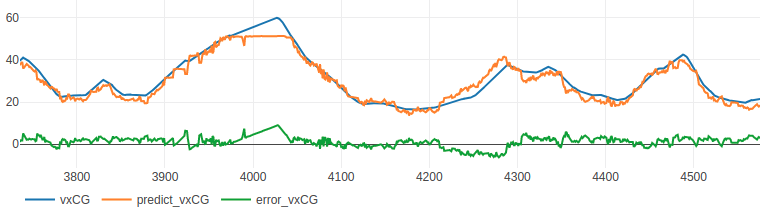
\includegraphics[width=\textwidth]{model80/zoom_vxCG.png}
\caption{Model 80 zoomed-in longitudinal velocity test set actual vs predicted.}
\label{fig:model80_zoom_vx}
\end{figure}

\begin{figure}[!ht]
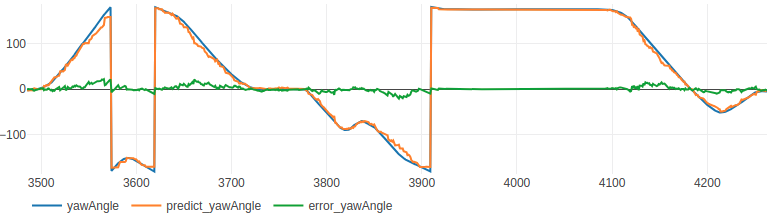
\includegraphics[width=\textwidth]{model80/zoom_yawAngle.png}
\caption{Model 80 zoomed-in yaw angle test set actual vs predicted.}
\label{fig:model80_zoom_yaw}
\end{figure}

\begin{figure}[!ht]
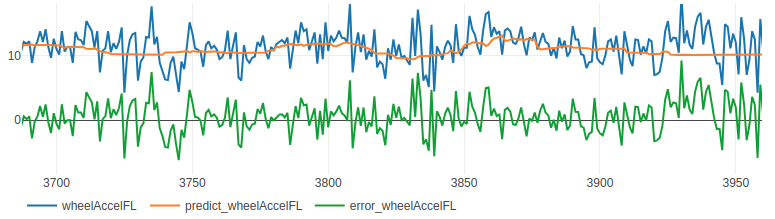
\includegraphics[width=\textwidth]{model80/zoom_wheelAccelFL.png}
\caption{Model 80 zoomed-in front left wheel acceleration test set actual vs predicted.}
\label{fig:model80_zoom_wheel}
\end{figure}

\section{Conclusion/Future Work }
From these results LSTM's outperformed attempts to hand engineer temporal relationships into the data then train with simple multi-layer networks, and LSTM models appear generally capable of learning vehicle dynamics with temporal delays. However, LSTM results still had a significant MSE between predicted future results and actual future results in the test set, so the investigated network architecture does not appear to be a candidate to threaten replacing hand modeling vehicle dynamics for simulation.

For future work I would like to investigate:
\begin{enumerate}
    \item \textbf{Integrating physical modeling with a RNN}: as proposed by \cite{shi2018neural, zeng2019tossingbot}. The approach proposed in both \cite{shi2018neural} and \cite{zeng2019tossingbot} is to utilize a physics model to implement the known features of movement then integrating with a learning model to fine-tune the unknown features or hardware unit specific features. Specifically, I would like to integrate a TensorFlow LSTM model with the PyBullet \cite{bullet} physics simulator's vehicle model, then apply common steering / brake / throttle input in simulation as from a real-world data capture and plot the resulting differences in position and orientation over time.
    \item \textbf{Predict movement farther into the future}: this project continually predicted only the next step of movement based on recent history, it would be interesting to understand how much future movement could be accurately predicted based on the recent past.
\end{enumerate}

\printbibliography

\section{Appendix}

\begin{appendices}
\section{Model Hyperparameters and Results}
X and Y data groups are defined in Appendix \ref{appendix:data}
\begin{longtable}{c | c | c | c | c | c | c | c | c | c | c | c | c}
ID & X & Y & dropout & rate & decay & time & norm & units & seq len & files & loss & mean error \\
1 & x1 & y1 & 0.1 & 0.02 & 0.0 & 0:08:22 & False & 10 & 10 & 1 & 12.05 & 1.47 \\
2 & x1 & y1 & 0.2 & 0.02 & 0.0 & 0:10:17 & False & 10 & 10 & 1 & 19.03 & 1.63 \\
3 & x1 & y1 & 0.0 & 0.02 & 0.0 & 0:10:46 & False & 10 & 10 & 1 & 84.33 & 3.23 \\
4 & x1 & y1 & 0.0 & 0.02 & 0.0 & 0:03:49 & True & 10 & 10 & 1 & 327.15 & 5.29 \\
5 & x1 & y1 & 0.0 & 0.02 & 0.0 & 0:06:36 & False & 10 & 10 & 1 & 8.86 & 1.36 \\
6 & x1 & y1 & 0.0 & 0.02 & 0.0 & 0:04:08 & True & 10 & 10 & 1 & 88.96 & 3.4 \\
7 & x1 & y1 & 0.1 & 0.02 & 0.0 & 0:11:04 & False & 10 & 10 & 1 & 11.65 & 1.43 \\
8 & x1 & y1 & 0.1 & 0.02 & 0.0 & 0:05:12 & True & 10 & 10 & 1 & 327.02 & 5.3 \\
9 & x1 & y1 & 0.1 & 0.02 & 0.0 & 0:04:49 & True & 10 & 10 & 1 & 64.09 & 2.67 \\
10 & x1 & y1 & 0.0 & 0.02 & 1e-06 & 0:04:49 & False & 10 & 10 & 1 & 21.29 & 1.96 \\
11 & x1 & y1 & 0.0 & 0.02 & 1e-06 & 0:03:16 & True & 10 & 10 & 1 & 326.67 & 5.28 \\
12 & x1 & y1 & 0.0 & 0.02 & 1e-06 & 0:07:00 & False & 10 & 10 & 1 & 11.55 & 1.5 \\
13 & x1 & y1 & 0.0 & 0.02 & 1e-06 & 0:04:09 & True & 10 & 10 & 1 & 42.52 & 2.58 \\
14 & x1 & y1 & 0.1 & 0.02 & 1e-06 & 0:10:32 & False & 10 & 10 & 1 & 12.07 & 1.5 \\
15 & x1 & y1 & 0.1 & 0.02 & 1e-06 & 0:02:22 & True & 10 & 10 & 1 & 327.1 & 5.3 \\
16 & x1 & y1 & 0.1 & 0.02 & 1e-06 & 0:07:21 & False & 10 & 10 & 1 & 12.4 & 1.5 \\
17 & x1 & y1 & 0.1 & 0.02 & 1e-06 & 0:05:17 & True & 10 & 10 & 1 & 49.21 & 2.61 \\
18 & x1 & y1 & 0.0 & 0.01 & 0.0 & 0:04:59 & False & 10 & 10 & 1 & 15.06 & 1.67 \\
19 & x1 & y1 & 0.0 & 0.01 & 0.0 & 0:05:09 & True & 10 & 10 & 1 & 229.6 & 4.31 \\
20 & x1 & y1 & 0.0 & 0.01 & 0.0 & 0:12:16 & False & 10 & 10 & 1 & 6.77 & 1.19 \\
21 & x1 & y1 & 0.0 & 0.01 & 0.0 & 0:07:28 & True & 10 & 10 & 1 & 18.41 & 1.85 \\
22 & x1 & y1 & 0.1 & 0.01 & 0.0 & 0:07:51 & False & 10 & 10 & 1 & 10.37 & 1.37 \\
23 & x1 & y1 & 0.1 & 0.01 & 0.0 & 0:03:28 & True & 10 & 10 & 1 & 326.39 & 5.3 \\
24 & x1 & y1 & 0.1 & 0.01 & 0.0 & 0:08:28 & False & 10 & 10 & 1 & 9.59 & 1.34 \\
25 & x1 & y1 & 0.1 & 0.01 & 0.0 & 0:06:05 & True & 10 & 10 & 1 & 21.2 & 1.84 \\
26 & x1 & y1 & 0.0 & 0.01 & 1e-06 & 0:06:54 & False & 10 & 10 & 1 & 9.99 & 1.42 \\
27 & x1 & y1 & 0.0 & 0.01 & 1e-06 & 0:13:04 & True & 10 & 10 & 1 & 25.53 & 2.18 \\
28 & x1 & y1 & 0.0 & 0.01 & 1e-06 & 0:12:38 & False & 10 & 10 & 1 & 6.63 & 1.16 \\
29 & x1 & y1 & 0.0 & 0.01 & 1e-06 & 0:11:11 & True & 10 & 10 & 1 & 10.68 & 1.48 \\
30 & x1 & y1 & 0.1 & 0.01 & 1e-06 & 0:19:28 & False & 10 & 10 & 1 & 8.36 & 1.27 \\
31 & x1 & y1 & 0.1 & 0.01 & 1e-06 & 0:08:55 & True & 10 & 10 & 1 & 20.14 & 1.8 \\
32 & x1 & y1 & 0.1 & 0.01 & 1e-06 & 0:15:04 & False & 10 & 10 & 1 & 8.31 & 1.25 \\
33 & x1 & y1 & 0.1 & 0.01 & 1e-06 & 0:09:15 & True & 10 & 10 & 1 & 15.58 & 1.65 \\
34 & x1 & y1 & 0.0 & 0.001 & 0.0 & 0:16:28 & False & 10 & 10 & 1 & 5.73 & 1.04 \\
35 & x1 & y1 & 0.0 & 0.001 & 0.0 & 0:27:15 & True & 10 & 10 & 1 & 6.5 & 1.13 \\
36 & x1 & y1 & 0.0 & 0.001 & 0.0 & 0:21:56 & False & 10 & 10 & 1 & 5.14 & 0.94 \\
37 & x1 & y1 & 0.0 & 0.001 & 0.0 & 0:26:26 & True & 10 & 10 & 1 & 5.69 & 1.04 \\
38 & x1 & y1 & 0.1 & 0.001 & 0.0 & 0:21:00 & False & 10 & 10 & 1 & 6.61 & 1.11 \\
39 & x1 & y1 & 0.1 & 0.001 & 0.0 & 0:29:52 & True & 10 & 10 & 1 & 7.55 & 1.21 \\
40 & x1 & y1 & 0.1 & 0.001 & 0.0 & 0:24:44 & False & 10 & 10 & 1 & 6.82 & 1.11 \\
41 & x1 & y1 & 0.1 & 0.001 & 0.0 & 0:30:47 & True & 10 & 10 & 1 & 7.49 & 1.2 \\
42 & x1 & y1 & 0.0 & 0.001 & 1e-06 & 0:17:31 & False & 10 & 10 & 1 & 5.53 & 1.01 \\
43 & x1 & y1 & 0.0 & 0.001 & 1e-06 & 0:29:00 & True & 10 & 10 & 1 & 6.13 & 1.09 \\
44 & x1 & y1 & 0.0 & 0.001 & 1e-06 & 0:20:38 & False & 10 & 10 & 1 & 5.16 & 0.96 \\
45 & x1 & y1 & 0.0 & 0.001 & 1e-06 & 0:24:18 & True & 10 & 10 & 1 & 5.95 & 1.08 \\
46 & x1 & y1 & 0.0 & 0.001 & 0.0 & 0:31:49 & False & 20 & 20 & 1 & 5.37 & 0.99 \\
47 & x2 & y1 & 0.1 & 0.001 & 1e-06 & 2:50:53 & False & 110 & 110 & 1 & 5.48 & 0.98 \\
48 & x2 & y2 & 0.2 & 0.002 & 1e-07 & 0:49:02 & False & 60 & 30 & 1 & 10.88 & 1.17 \\
49 & x1 & y2 & 0.1 & 0.001 & 0.0 & 1:40:20 & False & 100 & 100 & 1 & 8.67 & 1.07 \\
50 & x2 & y2 & 0.0 & 0.002 & 1e-06 & 0:31:11 & True & 200 & 100 & 1 & 646.85 & 7.69 \\
51 & x1 & y1 & 0.2 & 0.002 & 1e-06 & 1:35:48 & False & 90 & 90 & 1 & 7.41 & 1.15 \\
52 & x3 & y3 & 0.1 & 0.002 & 1e-07 & 1:32:49 & False & 70 & 70 & 3 & 9.16 & 1.28 \\
53 & x3 & y3 & 0.1 & 0.002 & 1e-06 & 3:02:05 & False & 160 & 160 & 4 & 7.71 & 1.17 \\
54 & x3 & y3 & 0.0 & 0.001 & 0.0 & 2:53:17 & False & 160 & 160 & 2 & 6.06 & 1.02 \\
55 & x3 & y3 & 0.1 & 0.002 & 1e-07 & 3:56:08 & False & 130 & 130 & 4 & 6.86 & 1.11 \\
56 & x3 & y3 & 0.0 & 0.001 & 1e-07 & 1:10:24 & False & 70 & 70 & 2 & 7.08 & 1.08 \\
57 & x3 & y3 & 0.2 & 0.005 & 1e-06 & 0:17:54 & False & 20 & 20 & 7 & 34.24 & 2.33 \\
58 & x3 & y3 & 0.1 & 0.005 & 1e-07 & 1:35:55 & False & 190 & 190 & 4 & 7.99 & 1.17 \\
59 & x3 & y3 & 0.0 & 0.005 & 1e-06 & 0:32:45 & False & 140 & 140 & 1 & 10.75 & 1.35 \\
60 & x3 & y3 & 0.2 & 0.008 & 1e-07 & 0:06:46 & False & 10 & 10 & 5 & 26.07 & 1.93 \\
61 & x3 & y3 & 0.0 & 0.008 & 1e-07 & 0:30:35 & False & 130 & 130 & 5 & 10.6 & 1.42 \\
62 & x3 & y3 & 0.1 & 0.005 & 1e-07 & 0:28:22 & False & 20 & 20 & 8 & 11.04 & 1.43 \\
63 & x3 & y3 & 0.0 & 0.008 & 1e-06 & 1:34:14 & False & 160 & 160 & 5 & 7.72 & 1.23 \\
64 & x3 & y3 & 0.1 & 0.008 & 1e-07 & 0:57:13 & False & 60 & 60 & 6 & 7.75 & 1.16 \\
65 & x3 & y3 & 0.0 & 0.008 & 1e-07 & 0:44:49 & False & 190 & 190 & 7 & 10.46 & 1.44 \\
66 & x3 & y3 & 0.1 & 0.008 & 1e-07 & 2:17:15 & False & 110 & 110 & 2 & 7.33 & 1.12 \\
67 & x3 & y3 & 0.0 & 0.005 & 1e-06 & 1:00:10 & False & 190 & 190 & 5 & 8.66 & 1.25 \\
68 & x3 & y4 & 0.1 & 0.005 & 1e-06 & 2:21:13 & False & 190 & 190 & 2 & 9.01 & 1.12 \\
69 & x3 & y4 & 0.2 & 0.008 & 1e-06 & 0:40:49 & False & 50 & 50 & 4 & 15.9 & 1.42 \\
70 & x3 & y4 & 0.2 & 0.005 & 1e-05 & 0:32:51 & False & 100 & 100 & 2 & 16.48 & 1.42 \\
71 & x3 & y4 & 0.2 & 0.005 & 1e-07 & 0:12:52 & False & 20 & 20 & 5 & 22.62 & 1.59 \\
72 & x3 & y4 & 0.1 & 0.005 & 1e-06 & 0:47:47 & False & 50 & 50 & 7 & 10.13 & 1.17 \\
73 & x3 & y4 & 0.1 & 0.008 & 1e-06 & 0:33:41 & False & 60 & 60 & 3 & 11.62 & 1.27 \\
74 & x3 & y4 & 0.1 & 0.008 & 1e-05 & 1:05:57 & False & 80 & 80 & 3 & 10.05 & 1.18 \\
75 & x3 & y4 & 0.2 & 0.005 & 1e-06 & 0:20:30 & False & 30 & 30 & 7 & 18.78 & 1.53 \\
76 & x3 & y4 & 0.1 & 0.008 & 1e-07 & 3:04:33 & False & 190 & 190 & 5 & 9.35 & 1.17 \\
77 & x3 & y4 & 0.2 & 0.005 & 1e-05 & 2:04:00 & False & 120 & 120 & 7 & 10.74 & 1.18 \\
78 & x3 & y4 & 0.2 & 0.008 & 1e-07 & 2:11:14 & False & 190 & 190 & 4 & 13.04 & 1.31 \\
79 & x3 & y4 & 0.1 & 0.008 & 1e-06 & 0:43:57 & False & 150 & 150 & 1 & 12.11 & 1.28 \\
80 & x3 & y4 & 0.1 & 0.005 & 1e-05 & 5:27:39 & False & 160 & 160 & 4 & 7.3 & 0.95 \\
81 & x3 & y4 & 0.2 & 0.008 & 1e-07 & 1:42:25 & False & 170 & 170 & 5 & 15.99 & 1.42 \\
82 & x3 & y4 & 0.2 & 0.008 & 1e-05 & 1:57:14 & False & 130 & 130 & 6 & 13.48 & 1.34 \\
83 & x3 & y4 & 0.2 & 0.008 & 1e-07 & 1:07:56 & False & 120 & 120 & 5 & 35.25 & 1.78 \\
84 & x3 & y4 & 0.1 & 0.005 & 1e-07 & 1:35:28 & False & 110 & 110 & 5 & 9.85 & 1.16 \\
85 & x3 & y4 & 0.0 & 0.008 & 1e-06 & 1:24:09 & False & 100 & 100 & 2 & 9.02 & 1.18 \\
86 & x3 & y4 & 0.1 & 0.005 & 1e-05 & 3:33:40 & False & 140 & 140 & 7 & 7.79 & 1.01 \\
87 & x3 & pitchAngle & 0.1 & 0.005 & 1e-05 & 1:06:52 & False & 200 & 200 & 4 & 0.02 & 0.11 \\
88 & x3 & wheelAccelRL & 0.1 & 0.001 & 0.0 & 0:06:14 & False & 200 & 200 & 4 & 83.33 & 8.51 \\
89 & x3 & vyCG & 0.1 & 0.005 & 1e-05 & 0:36:28 & False & 200 & 200 & 4 & 0.02 & 0.09 \\
90 & x3 & vyCG & 0.1 & 0.005 & 5e-05 & 0:36:22 & False & 200 & 200 & 4 & 0.02 & 0.09 \\
91 & x3 & vxCG & 0.1 & 0.005 & 1e-05 & 5:36:27 & False & 200 & 200 & 4 & 0.96 & 0.57 \\
92 & x3 & rollAngle & 0.1 & 0.005 & 1e-05 & 1:07:03 & False & 200 & 200 & 4 & 0.09 & 0.2 \\
93 & x3 & pitchAngle & 0.1 & 0.005 & 5e-05 & 0:42:32 & False & 200 & 200 & 4 & 0.03 & 0.11 \\
94 & x3 & rollAngle & 0.1 & 0.005 & 5e-05 & 1:37:12 & False & 200 & 200 & 4 & 0.04 & 0.14 \\
95 & x3 & vxCG & 0.1 & 0.005 & 5e-05 & 5:06:01 & False & 200 & 200 & 4 & 0.6 & 0.44 \\
96 & x3 & yawAngle & 0.1 & 0.005 & 1e-05 & 3:10:05 & False & 200 & 200 & 4 & 49.19 & 2.16 \\
97 & x3 & yawAngle & 0.1 & 0.005 & 3e-05 & 1:47:07 & False & 200 & 200 & 4 & 44.46 & 1.9 \\
98 & x3 & y5 & 0.1 & 0.005 & 3e-05 & 0:15:09 & False & 20 & 20 & 4 & 36.44 & 2.52 \\
99 & x3 & y6 & 0.1 & 0.005 & 1e-05 & 0:20:50 & False & 30 & 30 & 4 & 50.9 & 3.47 \\
100 & x4 & y6 & 0.1 & 0.005 & 3e-05 & 0:10:30 & False & 40 & 40 & 4 & 68.99 & 3.95 \\
101 & x4 & y6 & 0.1 & 0.005 & 3e-05 & 0:12:20 & False & 20 & 20 & 4 & 71.84 & 4.11 \\
102 & x4 & y6 & 0.1 & 0.005 & 3e-05 & 0:19:52 & False & 30 & 30 & 4 & 58.39 & 3.62 \\
103 & x4 & y6 & 0.1 & 0.005 & 1e-05 & 0:19:03 & False & 40 & 40 & 4 & 52.76 & 3.48 \\
104 & x4 & y6 & 0.1 & 0.005 & 5e-05 & 0:05:58 & False & 20 & 20 & 4 & 114.18 & 5.52 \\
105 & x4 & y6 & 0.1 & 0.005 & 5e-05 & 0:19:29 & False & 30 & 30 & 4 & 49.52 & 3.17 \\
106 & x4 & y6 & 0.1 & 0.005 & 1e-05 & 0:16:33 & False & 30 & 30 & 4 & 78.22 & 4.16 \\
107 & x4 & y6 & 0.1 & 0.005 & 5e-05 & 0:28:14 & False & 40 & 40 & 4 & 41.32 & 2.82 \\
108 & x4 & y6 & 0.1 & 0.005 & 1e-05 & 0:05:42 & False & 20 & 20 & 4 & 109.01 & 5.37 \\
\end{longtable}
\label{appendix:models}

\section{Data Set Groups}
\label{appendix:data}
\subsection{x1}
\label{appendix:datax1}
axCG, ayCG, azCG, brake, chassisAccelFL, chassisAccelFR, chassisAccelRL, chassisAccelRR, clutch, handwheelAngle, deflectionFL, deflectionFR, horizontalSpeed, pitchAngle, pitchRate, rollAngle, rollRate, throttle, vxCG, vyCG, vzCG, wheelAccelFL, wheelAccelFR, wheelAccelRL, wheelAccelRR, yawAngle, yawRate
\subsection{x2}
\label{appendix:datax2}
brake, clutch, handwheelAngle, throttle, horizontalSpeed, pitchAngle, pitchRate, rollAngle, rollRate, vxCG, vyCG, vzCG, yawAngle, yawRate
\subsection{x3}
\label{appendix:datax3}
brake, clutch, handwheelAngle, throttle, pitchAngle, pitchRate, rollAngle, rollRate, yawAngle, yawRate, vxCG, vyCG, vzCG, axCG, ayCG, azCG, wheelAccelFL, wheelAccelFR, wheelAccelRL, wheelAccelRR
\subsection{x4}
\label{appendix:datax4}
brake, clutch, handwheelAngle, throttle, pitchAngle, pitchRate, rollAngle, rollRate, yawAngle, yawRate, vxCG, vyCG, vzCG, axCG, ayCG, azCG
\subsection{y1}
\label{appendix:datay1}
axCG, ayCG, azCG, chassisAccelFL, chassisAccelFR, chassisAccelRL, chassisAccelRR, horizontalSpeed, pitchAngle, pitchRate, rollAngle, rollRate, vxCG, vyCG, vzCG, wheelAccelFL, wheelAccelFR, wheelAccelRL, wheelAccelRR, yawAngle, yawRate
\subsection{y2}
\label{appendix:datay2}
pitchAngle, rollAngle, vxCG, vyCG, vzCG, wheelAccelFL, wheelAccelFR, wheelAccelRL, wheelAccelRR, yawAngle
\subsection{y3}
\label{appendix:datay3}
pitchAngle, pitchRate, rollAngle, rollRate, yawAngle, yawRate, vxCG, vyCG, vzCG, axCG, ayCG, azCG, wheelAccelFL, wheelAccelFR, wheelAccelRL, wheelAccelRR
\subsection{y4}
\label{appendix:datay4}
pitchAngle, rollAngle, yawAngle, vxCG, vyCG, vzCG, wheelAccelFL, wheelAccelFR, wheelAccelRL, wheelAccelRR
\subsection{y5}
\label{appendix:datay5}
rollAngle, yawAngle, vxCG, vyCG, vzCG
\subsection{y6}
\label{appendix:datay6}
yawAngle, vxCG

\end{appendices}

\end{document}